%% bare_jrnl.tex
%% V1.4b
%% 2015/08/26
%% by Michael Shell
%% see http://www.michaelshell.org/
%% for current contact information.
%%
%% This is a skeleton file demonstrating the use of IEEEtran.cls
%% (requires IEEEtran.cls version 1.8b or later) with an IEEE
%% journal paper.
%%
%% Support sites:
%% http://www.michaelshell.org/tex/ieeetran/
%% http://www.ctan.org/pkg/ieeetran
%% and
%% http://www.ieee.org/

%%*************************************************************************
%% Legal Notice:
%% This code is offered as-is without any warranty either expressed or
%% implied; without even the implied warranty of MERCHANTABILITY or
%% FITNESS FOR A PARTICULAR PURPOSE! 
%% User assumes all risk.
%% In no event shall the IEEE or any contributor to this code be liable for
%% any damages or losses, including, but not limited to, incidental,
%% consequential, or any other damages, resulting from the use or misuse
%% of any information contained here.
%%
%% All comments are the opinions of their respective authors and are not
%% necessarily endorsed by the IEEE.
%%
%% This work is distributed under the LaTeX Project Public License (LPPL)
%% ( http://www.latex-project.org/ ) version 1.3, and may be freely used,
%% distributed and modified. A copy of the LPPL, version 1.3, is included
%% in the base LaTeX documentation of all distributions of LaTeX released
%% 2003/12/01 or later.
%% Retain all contribution notices and credits.
%% ** Modified files should be clearly indicated as such, including  **
%% ** renaming them and changing author support contact information. **
%%*************************************************************************


% *** Authors should verify (and, if needed, correct) their LaTeX system  ***
% *** with the testflow diagnostic prior to trusting their LaTeX platform ***
% *** with production work. The IEEE's font choices and paper sizes can   ***
% *** trigger bugs that do not appear when using other class files.       ***                          ***
% The testflow support page is at:
% http://www.michaelshell.org/tex/testflow/



\documentclass[journal]{IEEEtran}
%
% If IEEEtran.cls has not been installed into the LaTeX system files,
% manually specify the path to it like:
% \documentclass[journal]{../sty/IEEEtran}





% Some very useful LaTeX packages include:
% (uncomment the ones you want to load)

\usepackage{amsmath}

% *** MISC UTILITY PACKAGES ***
%
%\usepackage{ifpdf}
% Heiko Oberdiek's ifpdf.sty is very useful if you need conditional
% compilation based on whether the output is pdf or dvi.
% usage:
% \ifpdf
%   % pdf code
% \else
%   % dvi code
% \fi
% The latest version of ifpdf.sty can be obtained from:
% http://www.ctan.org/pkg/ifpdf
% Also, note that IEEEtran.cls V1.7 and later provides a builtin
% \ifCLASSINFOpdf conditional that works the same way.
% When switching from latex to pdflatex and vice-versa, the compiler may
% have to be run twice to clear warning/error messages.






% *** CITATION PACKAGES ***
%
%\usepackage{cite}
% cite.sty was written by Donald Arseneau
% V1.6 and later of IEEEtran pre-defines the format of the cite.sty package
% \cite{} output to follow that of the IEEE. Loading the cite package will
% result in citation numbers being automatically sorted and properly
% "compressed/ranged". e.g., [1], [9], [2], [7], [5], [6] without using
% cite.sty will become [1], [2], [5]--[7], [9] using cite.sty. cite.sty's
% \cite will automatically add leading space, if needed. Use cite.sty's
% noadjust option (cite.sty V3.8 and later) if you want to turn this off
% such as if a citation ever needs to be enclosed in parenthesis.
% cite.sty is already installed on most LaTeX systems. Be sure and use
% version 5.0 (2009-03-20) and later if using hyperref.sty.
% The latest version can be obtained at:
% http://www.ctan.org/pkg/cite
% The documentation is contained in the cite.sty file itself.


\usepackage{matlab-prettifier}


% *** GRAPHICS RELATED PACKAGES ***
%
\ifCLASSINFOpdf
  \usepackage[pdftex]{graphicx}
  % declare the path(s) where your graphic files are
  % \graphicspath{{../pdf/}{../jpeg/}}
  % and their extensions so you won't have to specify these with
  % every instance of \includegraphics
  % \DeclareGraphicsExtensions{.pdf,.jpeg,.png}
\else
  % or other class option (dvipsone, dvipdf, if not using dvips). graphicx
  % will default to the driver specified in the system graphics.cfg if no
  % driver is specified.
  % \usepackage[dvips]{graphicx}
  % declare the path(s) where your graphic files are
  % \graphicspath{{../eps/}}
  % and their extensions so you won't have to specify these with
  % every instance of \includegraphics
  % \DeclareGraphicsExtensions{.eps}
\fi
% graphicx was written by David Carlisle and Sebastian Rahtz. It is
% required if you want graphics, photos, etc. graphicx.sty is already
% installed on most LaTeX systems. The latest version and documentation
% can be obtained at: 
% http://www.ctan.org/pkg/graphicx
% Another good source of documentation is "Using Imported Graphics in
% LaTeX2e" by Keith Reckdahl which can be found at:
% http://www.ctan.org/pkg/epslatex
%
% latex, and pdflatex in dvi mode, support graphics in encapsulated
% postscript (.eps) format. pdflatex in pdf mode supports graphics
% in .pdf, .jpeg, .png and .mps (metapost) formats. Users should ensure
% that all non-photo figures use a vector format (.eps, .pdf, .mps) and
% not a bitmapped formats (.jpeg, .png). The IEEE frowns on bitmapped formats
% which can result in "jaggedy"/blurry rendering of lines and letters as
% well as large increases in file sizes.
%
% You can find documentation about the pdfTeX application at:
% http://www.tug.org/applications/pdftex

\usepackage{url}
\usepackage{hyperref}

% correct bad hyphenation here
\hyphenation{op-tical net-works semi-conduc-tor}


\begin{document}
%
% paper title
% Titles are generally capitalized except for words such as a, an, and, as,
% at, but, by, for, in, nor, of, on, or, the, to and up, which are usually
% not capitalized unless they are the first or last word of the title.
% Linebreaks \\ can be used within to get better formatting as desired.
% Do not put math or special symbols in the title.
\title{Thermoelectric Generator Characterization}
%
%
% author names and IEEE memberships
% note positions of commas and nonbreaking spaces ( ~ ) LaTeX will not break
% a structure at a ~ so this keeps an author's name from being broken across
% two lines.
% use \thanks{} to gain access to the first footnote area
% a separate \thanks must be used for each paragraph as LaTeX2e's \thanks
% was not built to handle multiple paragraphs
%

\author{Filippo~Faccini,~\IEEEmembership{241479} \\
Giacomo~Mazzucchi,~\IEEEmembership{248440}
}% <-this % stops a space



% note the % following the last \IEEEmembership and also \thanks - 
% these prevent an unwanted space from occurring between the last author name
% and the end of the author line. i.e., if you had this:
% 
% \author{....lastname \thanks{...} \thanks{...} }
%                     ^------------^------------^----Do not want these spaces!
%
% a space would be appended to the last name and could cause every name on that
% line to be shifted left slightly. This is one of those "LaTeX things". For
% instance, "\textbf{A} \textbf{B}" will typeset as "A B" not "AB". To get
% "AB" then you have to do: "\textbf{A}\textbf{B}"
% \thanks is no different in this regard, so shield the last } of each \thanks
% that ends a line with a % and do not let a space in before the next \thanks.
% Spaces after \IEEEmembership other than the last one are OK (and needed) as
% you are supposed to have spaces between the names. For what it is worth,
% this is a minor point as most people would not even notice if the said evil
% space somehow managed to creep in.


% The paper headers
%\markboth{Journal of \LaTeX\ Class Files,~Vol.~14, No.~8, August~2015}%
%{Shell \MakeLowercase{\textit{et al.}}: Bare Demo of IEEEtran.cls for IEEE Journals}
% The only time the second header will appear is for the odd numbered pages
% after the title page when using the twoside option.
% 
% *** Note that you probably will NOT want to include the author's ***
% *** name in the headers of peer review papers.                   ***
% You can use \ifCLASSOPTIONpeerreview for conditional compilation here if
% you desire.




% If you want to put a publisher's ID mark on the page you can do it like
% this:
%\IEEEpubid{0000--0000/00\$00.00~\copyright~2015 IEEE}
% Remember, if you use this you must call \IEEEpubidadjcol in the second
% column for its text to clear the IEEEpubid mark.



% use for special paper notices
%\IEEEspecialpapernotice{(Invited Paper)}


% make the title area
\maketitle

% As a general rule, do not put math, special symbols or citations
% in the abstract or keywords.
\begin{abstract}
  {T}{hermoelectric} generators (TEGs) are solid-state devices that exploit the Seebeck effect to generate electric current from a temperature difference. The objective of this paper is to develop an automated system to collect data on TEGs and characterize the internal resistance and Seebeck coefficient of a new fiber-based flexible TEG design.
  % Thermoelectric generator. We developed an automatic system to gather the data
   % The realization of a new type of TEG always requires characterization to validate behaviour and efficiency. TEGs are generally modeled as a voltage generator with an internal series resistance, the purpose of characterization is to find the relationship between temperature delta and power output taking into account the internal resistance of the generator.
\end{abstract}

% Note that keywords are not normally used for peerreview papers.
%\begin{IEEEkeywords}
%IEEE, IEEEtran, journal, \LaTeX, paper, template.
%\end{IEEEkeywords}

% For peer review papers, you can put extra information on the cover
% page as needed:
% \ifCLASSOPTIONpeerreview
% \begin{center} \bfseries EDICS Category: 3-BBND \end{center}
% \fi
%
% For peerreview papers, this IEEEtran command inserts a page break and
% creates the second title. It will be ignored for other modes.
\IEEEpeerreviewmaketitle



\section{Introduction}
% The very first letter is a 2 line initial drop letter followed
% by the rest of the first word in caps.
% 
% form to use if the first word consists of a single letter:
% \IEEEPARstart{A}{demo} file is ....
% 
% form to use if you need the single drop letter followed by
% normal text (unknown if ever used by the IEEE):
% \IEEEPARstart{A}{}demo file is ....
% 
% Some journals put the first two words in caps:
% \IEEEPARstart{T}{his demo} file is ....
% 
% Here we have the typical use of a "T" for an initial drop letter
% and "HIS" in caps to complete the first word.

% Context of the work

\IEEEPARstart{T}{EG} are mainly used in the context of energy harvesting, both on an industrial scale (generally large amounts of energy from chemical reactions) and for low power electronic devices (e.g., batteryless or hybrid systems). Wearable electronics, i.e., powering devices with body heat, is becoming popular in this field. However, having rigid TEGs was a limitation for developments in this field, as they are particularly uncomfortable when worn, a problem solved by the development of \textbf{flexible TEG modules} ~\cite{flexibletegc}. These use fiber-based materials that allow the TEG to be bent and adapted to curved surfaces, such as an arm.
\\
Currently, the TEG model we received has no characterization, so it is not possible to know how it behaves in terms of efficiency and power generated.
Characterization is essential to understand how the TEG behaves under real conditions and to be able to use it in a power generation system.
The efficiency of a TEG is governed by the dimensionless figure of merit \textbf{Zero Temperature Difference} (\textbf{ZT}), which depends on the material's \textbf{Seebeck coefficient, electrical conductivity and thermal conductivity}.
Improvements in any of these parameters can lead to enhanced performance, but they often involve trade-offs, such as increased electrical conductivity leading to higher thermal conductivity, which can reduce the temperature gradient needed for power generation.
The ideal TEG has a high Seebeck coefficient, high electrical conductivity, and low thermal conductivity.
The best way to characterize a TEG is to \textbf{measure the open-circuit voltage and the current generated with a load resistor}. 
These data can be used to fit the Seebeck model and find the internal parameters of the TEG. 



\section{Related Work}
The most complete work on TEG is the paper of Tohidi, Holagh and Chitsaz ~\cite{TOHIDI2022117793} where the authors describe in details the working principle of TEG, the efficiency and the limitations of these devices, starting from thermodynamics principles then focusing on fabrication designs, modeling the TEG as a semiconductor device (also in ~\cite{Tian16}). One of the most relevant statements is that the \textbf{maximum output power of a TEG is achieved when the load resistance equals the internal resistance of the module}, useful when designing actual circuits or find the maximum efficiency of the TEG (related to the figure of merit). Then they explore the possible applications, especially in industrial processes and in the automotive sector (e.g., recovering waste heat from the engine).
\\
We found 3 examples of TEG characterization in the literature, which basically follow the same principles with minor variations.

\begin{itemize}
  \item Oswaldo Hideo Ando Junior, Nelson H. Calderon and Samara Silva de Souza developed in their work ~\cite{en11061555} a system to recover the energy from the waste heat of industrial processes. In these cases, the temperature difference is quite high, so the TEG can generate a significant amount of power. In particular they used a configuration of 10 TEG modules in series and 20 in parallel, reaching a \textbf{maximum power output of 29W} with a temperature difference of 80°C.
  \item The same strategy was employed by \cite{CARMO20112194} for characterization, namely measuring with an open circuit and a load resistor. The resulting model of the TEG was linear, both for the internal resistance and the Seebeck coefficient. Ultimately, the \textbf{SPICE model} of the TEG was obtained, thus enabling its use in simulations. 
  \item Finally, ~\cite{10209119} uses also the same approach, with the additional collection of data regarding thermal conductivity. Their methodology was based on steady-state principles, specifically \textbf{insulating the TEG with the heater} and logging the energy required to heat the TEG under load.   
\end{itemize}

\section{Description of the work for the project}
The project was divided into two parts: \textbf{developing an automatic system} to get the TEG measurements and \textbf{fitting the data} to find the TEG parameters.
To have a complete characterization, two types of data are needed: the open-circuit voltage that is measured at the ends of the TEG when a temperature difference is applied and the current that flows through a load resistor.

The tools needed for the acquisition are the following:
\begin{itemize}
  \item The \textbf{STM32 NUCLEO-F401RE board}.
  \item The \textbf{heating and cooling control circuit board}. We used a prototype board on a matrix board.
  \item \textbf{One TEG module} with fan and heatsink on one side and the heating resistor on the other one.
  \item \textbf{Two thermocouples} (installed on the hot and cold sides). We used the \href{https://www.analog.com/media/en/technical-documentation/data-sheets/MAX6675.pdf}{MAX6675 module}.
  \item \textbf{One bench power supply} (at least rated at \(40 W\)).
  \item A PC with our \textbf{GUI application} to control MCU settings.
\end{itemize}

\begin{figure}[h]
  \centering
  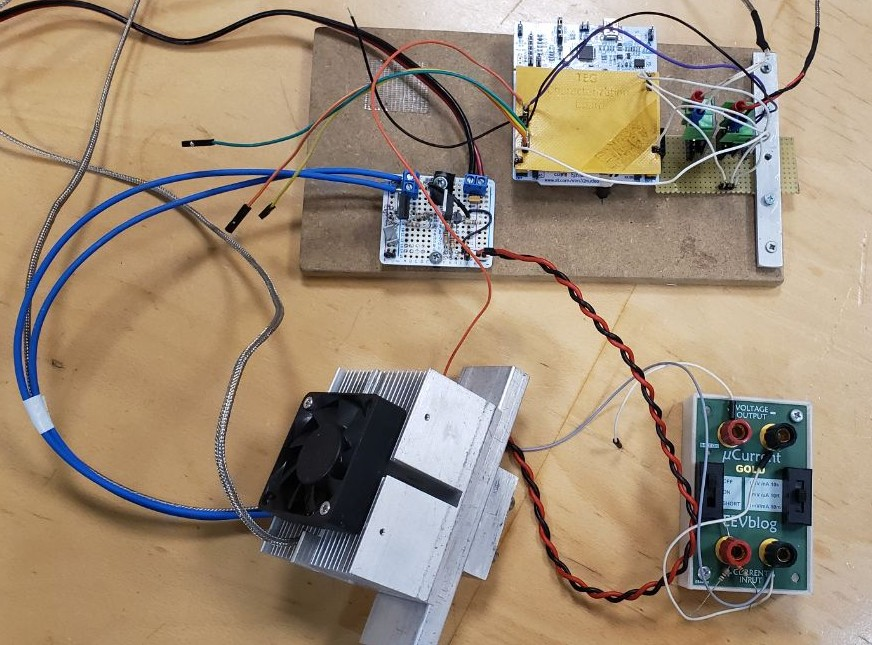
\includegraphics[width=0.45\textwidth]{assets/all_project_photo2.jpg}
  \caption{A photo of the used materials}
\end{figure}

The data acquisition procedure is organized as follows.
\begin{enumerate}
  \item Power the heating and cooling circuit, connect the STM32 NUCLEO board to the PC and open the control GUI.
  \item Set the two target temperatures from the PC and start.
  \item Save the acquired data (voltages, currents and temperatures) in CSV format on the PC.
\end{enumerate}

The STM32 uses the UART in DMA mode to communicate with the PC, the SPI to read data from the thermocouples (\href{https://www.analog.com/media/en/technical-documentation/data-sheets/MAX6675.pdf}{MAX6675 module}), the ADC to read the voltage from the TEGC, and the PWMs to control the fan and temperature of the heating resistor.

\subsection{Measurements}
TEG characterization requires us to estimate the Seebeck coefficient and the internal resistance. The method we used allowed us to estimate the two parameters with two different type of measurements.
The first one is the open-circuit voltage measurement, which allows us to estimate the Seebeck coefficient. The second one is the current measurement, which is needed to define the internal resistance. In this second test we depend on the already estimated Seebeck coefficient.

\subsection{Voltage open circuit measurement (VOC)}
\label{sec:voc-measurement}

\begin{figure}[h]
  \centering
  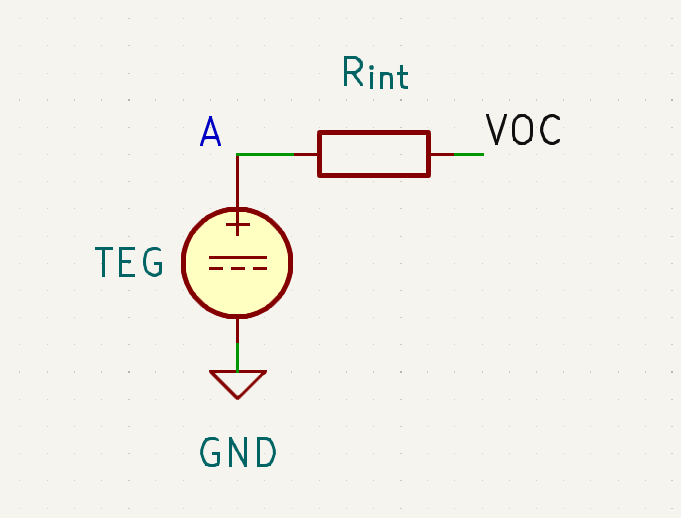
\includegraphics[width=0.45\textwidth]{assets/VOC_circuit.png}
  \caption{TEG model in open circuit configuration}
  \label{fig:oc_model}
\end{figure}
\begin{figure}[h]
  \centering
  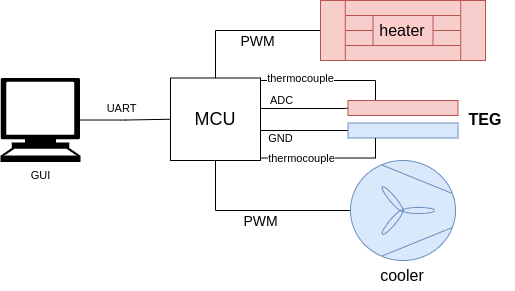
\includegraphics[width=0.45\textwidth]{assets/VOC_schema.png}
  \caption{Open circuit voltage measurement diagram}
\end{figure}

The open-circuit voltage (VOC) is the voltage measured at the ends of the TEG with no load connected, in our case, we can measure a voltage only when there is a temperature difference between the TEG surfaces.
With this test we want to measure the voltage generation of the TEG alone, and neglect the effect of the internal resistance. The only way to measure point A in figure \ref{fig:oc_model}, is to have zero current passing through $R_{int}$. To make a measurement without absorbing current, we can exploit the fact that the ADC is constructed to have high impedance, and so will limit the current to $ 5 nA $. With this in mind we can neglect this currents and assume that the measurement is done directly in point A.\\
TEG voltage is generated by the Seebeck effect, and it is proportional to the temperature difference between the hot and cold sides of the TEG, so with this test we can directly estimate the coefficient without considering other factors.
\\
The VOC is given by the following equation:

\begin{equation}
  V_{OC} = S \cdot \Delta T
  \label{eq:voc}
\end{equation}

where $ S $ is the Seebeck coefficient of the TEG and $ \Delta T $ is the temperature difference between the hot and cold sides.
The Seebeck coefficient is a material property that characterizes the voltage generated by a temperature difference, it will be used to calculate the power outut of the TEG.

\subsection{Current measurement}

\begin{figure}[h]
  \centering
  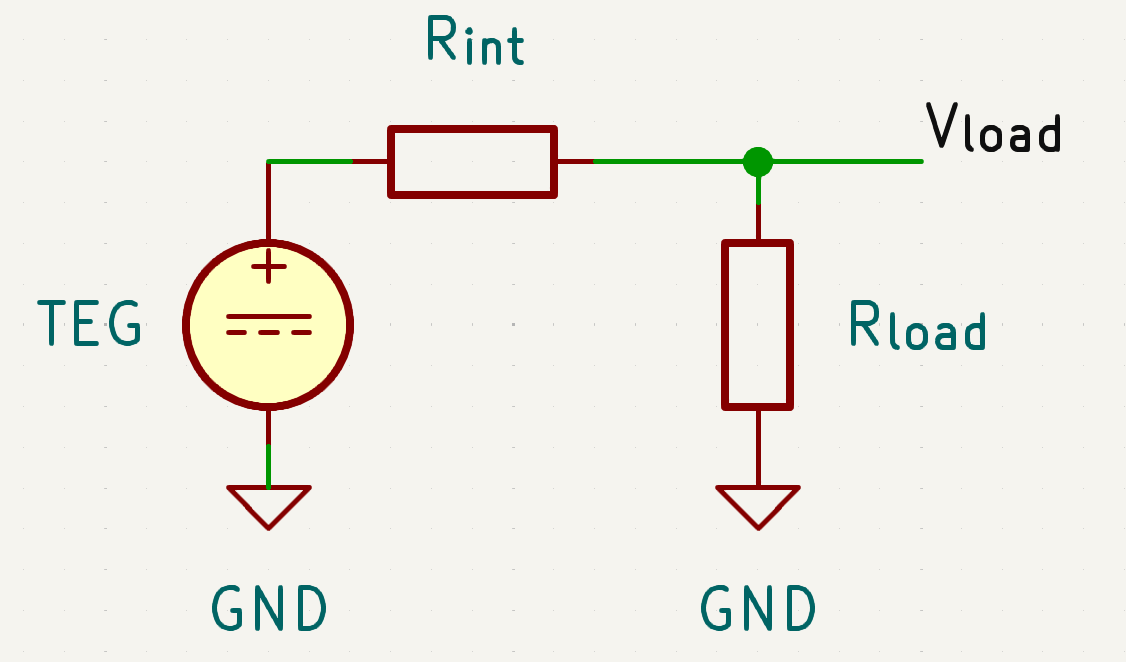
\includegraphics[width=0.45\textwidth]{assets/load_circuit.png}
  \caption{TEG model with a resistive load}
\end{figure}

The current generated by the TEG can be measured by attaching a known load resistor to the TEG and is described by the following equation:

\begin{equation}
  I = \frac{V_{OC}}{R_{int} + R_{load}}
\end{equation}

where $I$ is the current generated by the TEG, $ V_{OC} $ is the open-circuit voltage of the TEG, $ R_{int} $ is the internal resistance of the TEG, and $ R_{load} $ is the load resistor attached to the TEG.
\\
In the equation the only unknown is $R_{int}$ in fact the load resistance is chosen, $ I $ is the measured quantity and $ V_{OC} $ is instead calculated by equation \ref{eq:voc}.\\
The difficult part is to do the current measurement from the microcontroller, in fact it has no direct interface to measure it, so one way is to measure the voltage drop on a known resistance, and use $ I =  \frac{\Delta V}{R} $ to calculate the current. A shunt is a device that does this exact thing. The microcontroller's ADC has a resolution of 12 bits and the voltages are between 0 and 3.3, so, as shown here \ref{eq:adc_calculation}, the resolution is of $ 0.8 mV $.

\begin{equation}
  Resolution = \frac{3.3 V}{2^{12}} = \frac{3.3 V}{4096} = \approx 0.0008 V
  \label{eq:adc_calculation}
\end{equation}

To effectively measure we used an external module, the \href{https://www.eevblog.com/projects/ucurrent/}{\textbf{microCurrent}}, to amplify the signal then read by the MCU's ADC. This module has a tunable amplification circuit that allows to change the expected scale and resolution to fit the expected currents range.

\begin{figure}[h]
  \centering
  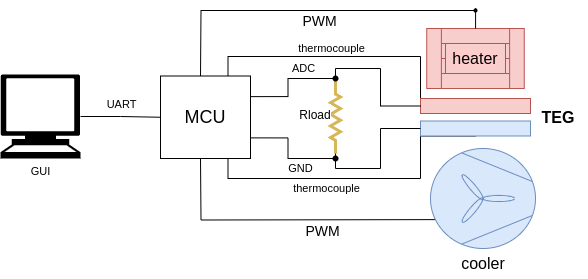
\includegraphics[width=0.45\textwidth]{assets/load_schema.png}
  \caption{Current measurement diagram with a resistive load}
\end{figure}


\subsection{Hot side temperature control}

\begin{figure}
  \centering
  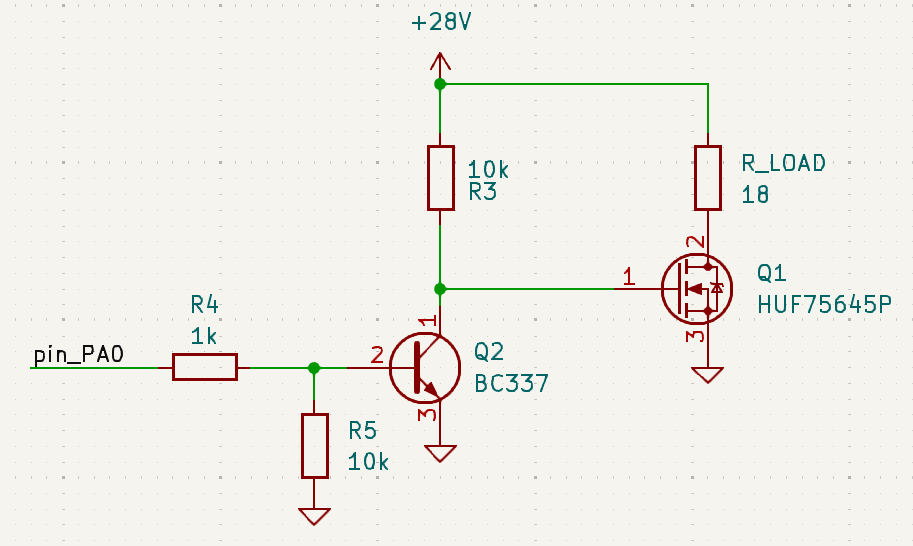
\includegraphics[width=0.45\textwidth]{assets/heat_control.png}
  \caption{Current control circuit}
  \label{fig:heat_control}
\end{figure}

For every measurement we need a temperature difference between the two sides of the TEG, so we
need to control the temperature of the hot side.
We used a \textbf{wire wound resistor with a current control}. The circuit (in Figure \ref{fig:heat_control}) involves a \href{https://www.onsemi.com/pdf/datasheet/huf75645s3s-d.pdf}{MOSFET} driven by a \href{https://diotec.com/request/datasheet/bc337.pdf}{NPN transistor}. As a load resistor we used a wire wound resistor of 18 effective ohms (measured with the multimeter). Both SPICE simulation and actual measurements confirm a maximum current of $ 1.4 A $ on the load resistor, with a maximum power around $ 35 W $ as shown here \ref{eq:power_supply_rating}. \\

\begin{equation}
  (1.4A)^2 * 18\Omega = 35W
  \label{eq:power_supply_rating}
\end{equation}

The circuit has reverse logic, so when the MCU pin is grounded the mosfet is activated and 1.4 A of current flows through, but when it is at 3.3V it stops. R3 and R5 are chosen according to this configuration, R4 is only a protection resistor for the MCU pin.


\subsection{Cold side temperature control}

To maintain a constant temperature, a \textbf{heatsink} was positioned on the cold side of the TEG. Subsequently, a fan was incorporated into the system to facilitate cooling of the aluminum, which proved particularly advantageous during steady-state acquisitions. This approach enabled the temperature of the hot side to be maintained at a stable level through the PID on the heater, the temperature of the cold side to be kept stable by the fan, and the delta to remain constant. A 12V fan with a PWM control was utilized. The power supply was the same as that used for the heater, and a \href{https://www.ti.com/lit/ds/symlink/lm317l.pdf}{voltage regulator} with the appropriate resistors was employed to provide a 12V power supply. The PID was tuned to control the fan, but we found out that it was preferable to run the fan constantly in steady-state measurements or to turn it off in measurements with equal delta temperatures but different average temperatures. 

\begin{figure}[h]
  \centering
  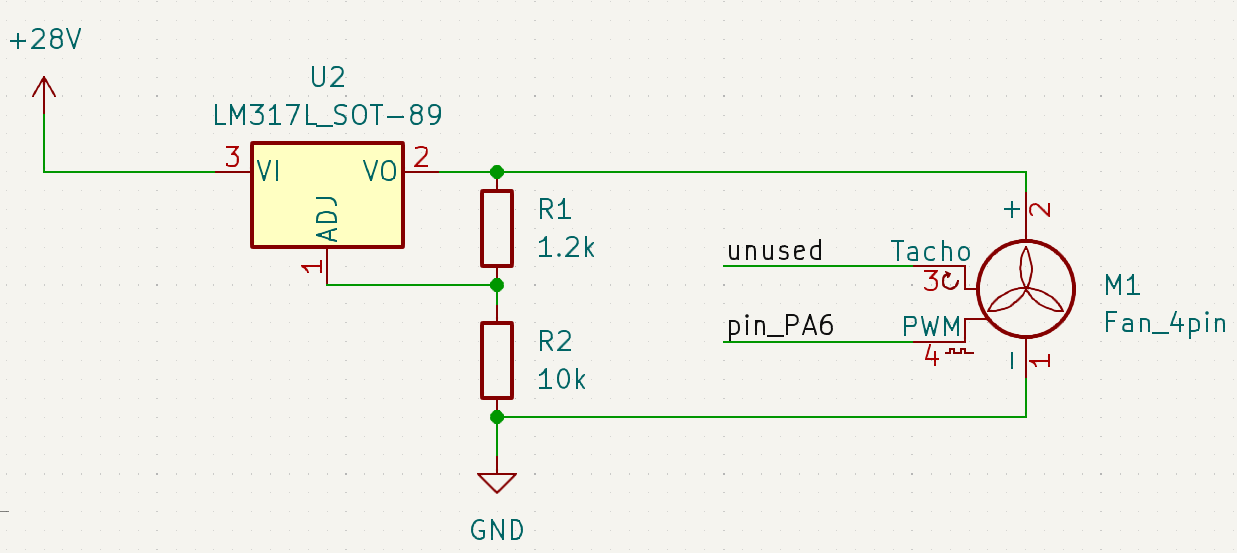
\includegraphics[scale=0.25]{assets/cooling_control.png}
  \caption{Cooling control circuit}
\end{figure}

\subsection{Acquisition process}

The MCU accepts via UART the following commands:
\begin{itemize}
  \item \textbf{setpoint hot\_side}: set the hot side temperature in Celsius degrees
  \item \textbf{duty duty\_cycle}: set the duty cycle of the PWM controlling the fan, from 0 to 1
  \item \textbf{pid kp ki kd}: set the PID parameters
\end{itemize}

The GUI application was developed in C++ using the \href{https://github.com/ocornut/imgui}{\textbf{Dear ImGui}} library and it allows to control the MCU parameters, plot the acquired data and save it in CSV format.

\begin{figure}[h]
  \centering
  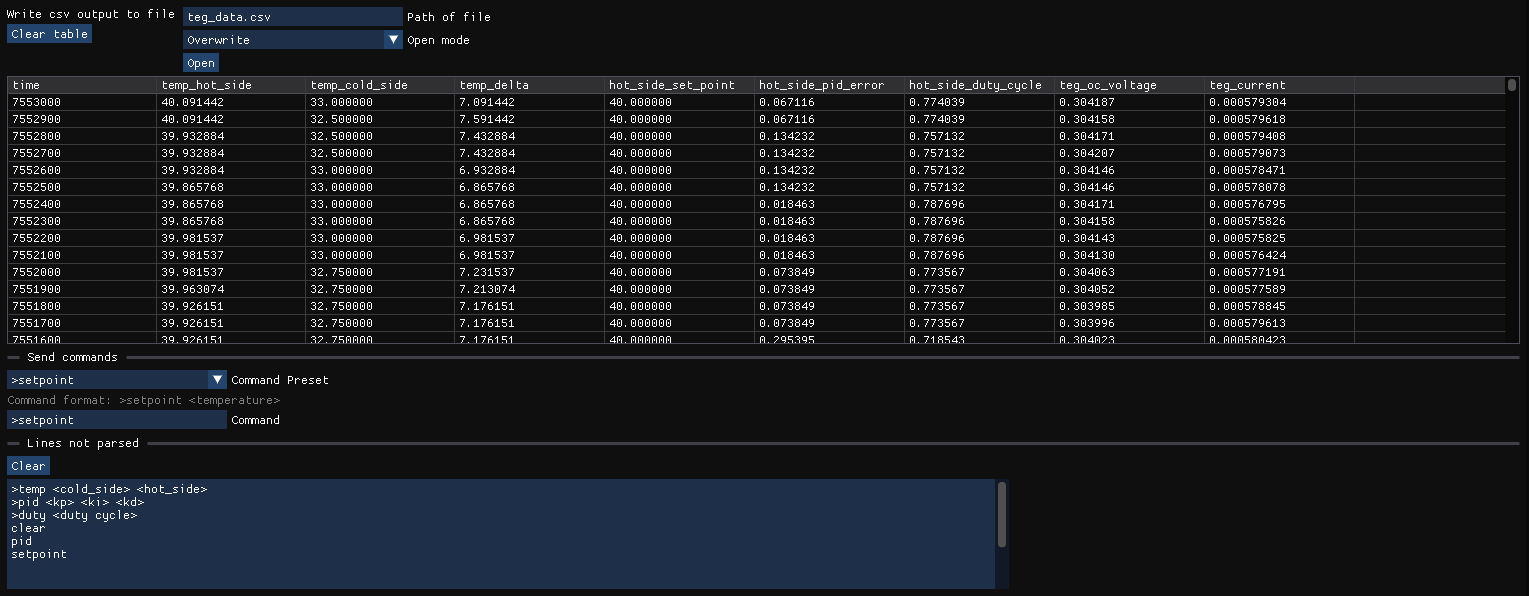
\includegraphics[width=0.5\textwidth]{assets/app_csv_commands.png}
  \caption{Sending the settings to the MCU}
\end{figure}

We carried out the acquisitions in the same environment, thus maintaining the same conditions for all acquisitions. We justify the time used for the development of the application as it was very useful both for acquiring accurate data and for quickly noticing any errors or dirty data so that we could stop and correct, saving time later.

\begin{figure}[h]
  \centering
  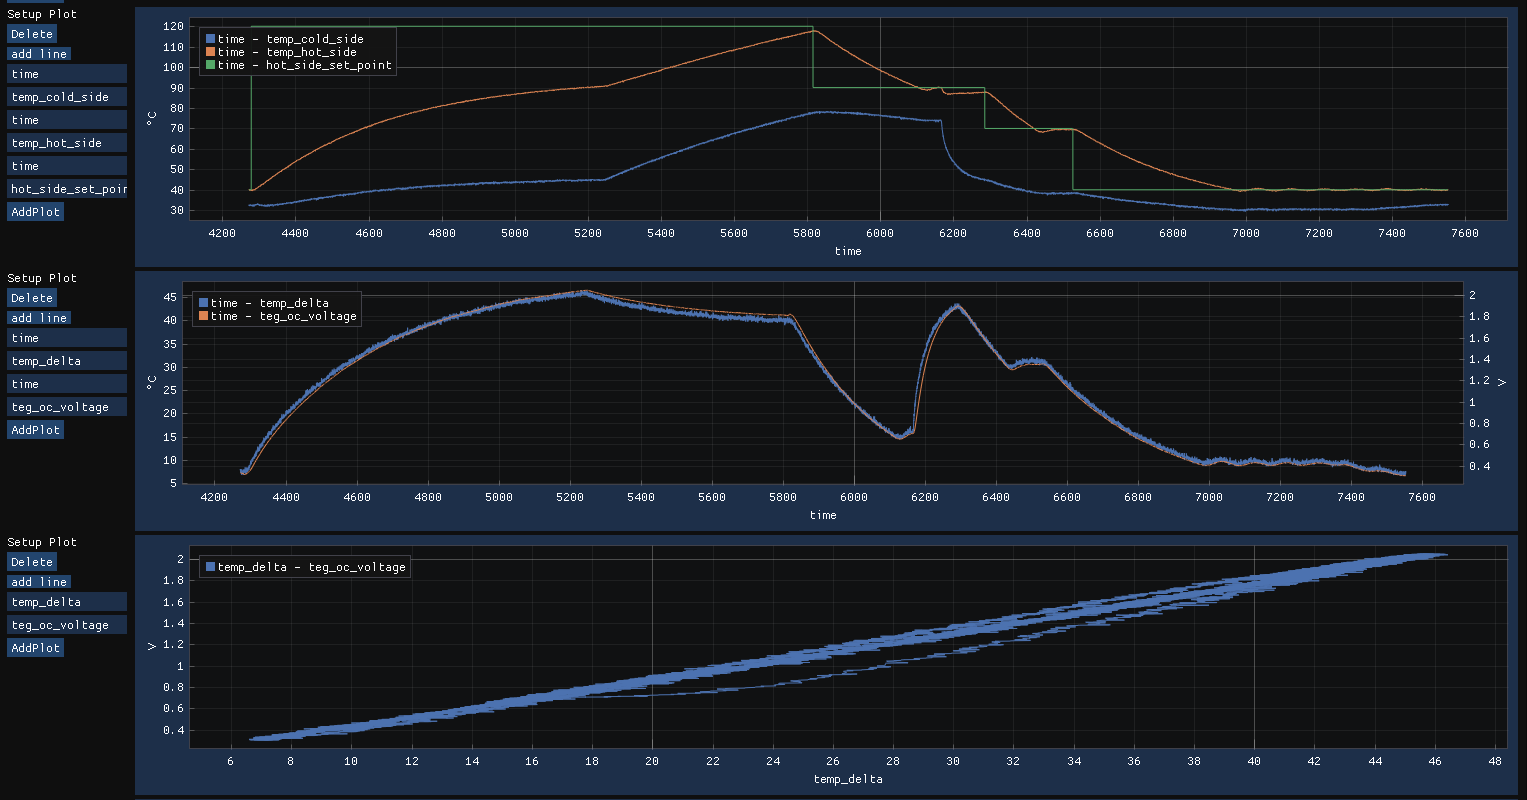
\includegraphics[width=0.5\textwidth]{assets/app_plots.png}
  \caption{Real time plots from the GUI application}
\end{figure}




\section{Experimental results}
% Add a Section about experimental results and verification of your output. 

% Any number, both final and intermediate results should be described. Even the experimental setup, and the measurement environment should be described. The measure should be reproducible by the readers. Listing the models of the instrument is not important (e.g.,  oscilloscope TD98445.... ), while the type of instrumentation or the type of measure is fundamental to repeat the experiment. \\
% \\
% In case, please, provide a shared folder (e.g., github, gitlab, Google Drive, ... ) where the code is available for repeat the experiments, the achieved results are available for a comparison. 

% The aim of this project was to identify the parameters of the different TEC modules and define which was the optimal one for the given application.
We estimate the internal resistance and the Seeback coefficient with a MATLAB script.
\subsection{Fitting Seeback coefficient}

The \textbf{Seebeck coefficient} (also known as thermopower, thermoelectric power, and thermoelectric sensitivity) of a material is a measure of the magnitude of an induced thermoelectric voltage in response to a temperature difference across that material, as induced by the Seebeck effect \cite{seebeckCoefficientWikipedia}, which is described by the equation \ref{eq:seeback}. It is one of the components of the figure of merit, which measures the overall efficiency of a thermoelectric device.

\begin{equation}
    S = \frac{ \Delta V}{\Delta T }
    \label{eq:seeback}
\end{equation}

As described in section \ref{sec:voc-measurement}, we can assume that we are measuring directly point A in figure \ref{fig:oc_model}. In this way, the voltage measured is dependent only on the Seeback coefficient, which in itself depends on the delta temperature between hot and cold. In MATLAB the model is written as follows:

\begin{lstlisting}[
    frame=single,
    numbers=none,
    style=Matlab-editor,
    basicstyle=\tiny,
]
% Seeback inline function
% T is a vector of mean temperature between hot and cold surfaces
seeback_coeff_mdl = @(coeffs, T)(coeffs(1));
% Model of the Open Circuit Voltage
voc_mdl = @(seeback_coeffs, T)(seeback_coeff_mdl(seeback_coeffs, T(:,1)) .* T(:,2));
% Create data table
tbl = table(mean_surface_temperature, delta_surface_temperature, measured_voltage);
% Fit model with initial guesses for each coefficient
nlm = fitnlm(tbl, voc_mdl, [0.0, 0.01, 0.02, 0.01],'Options',statset('Display','final','Robust','On'));
\end{lstlisting}

\begin{figure}[h]
    \centering
    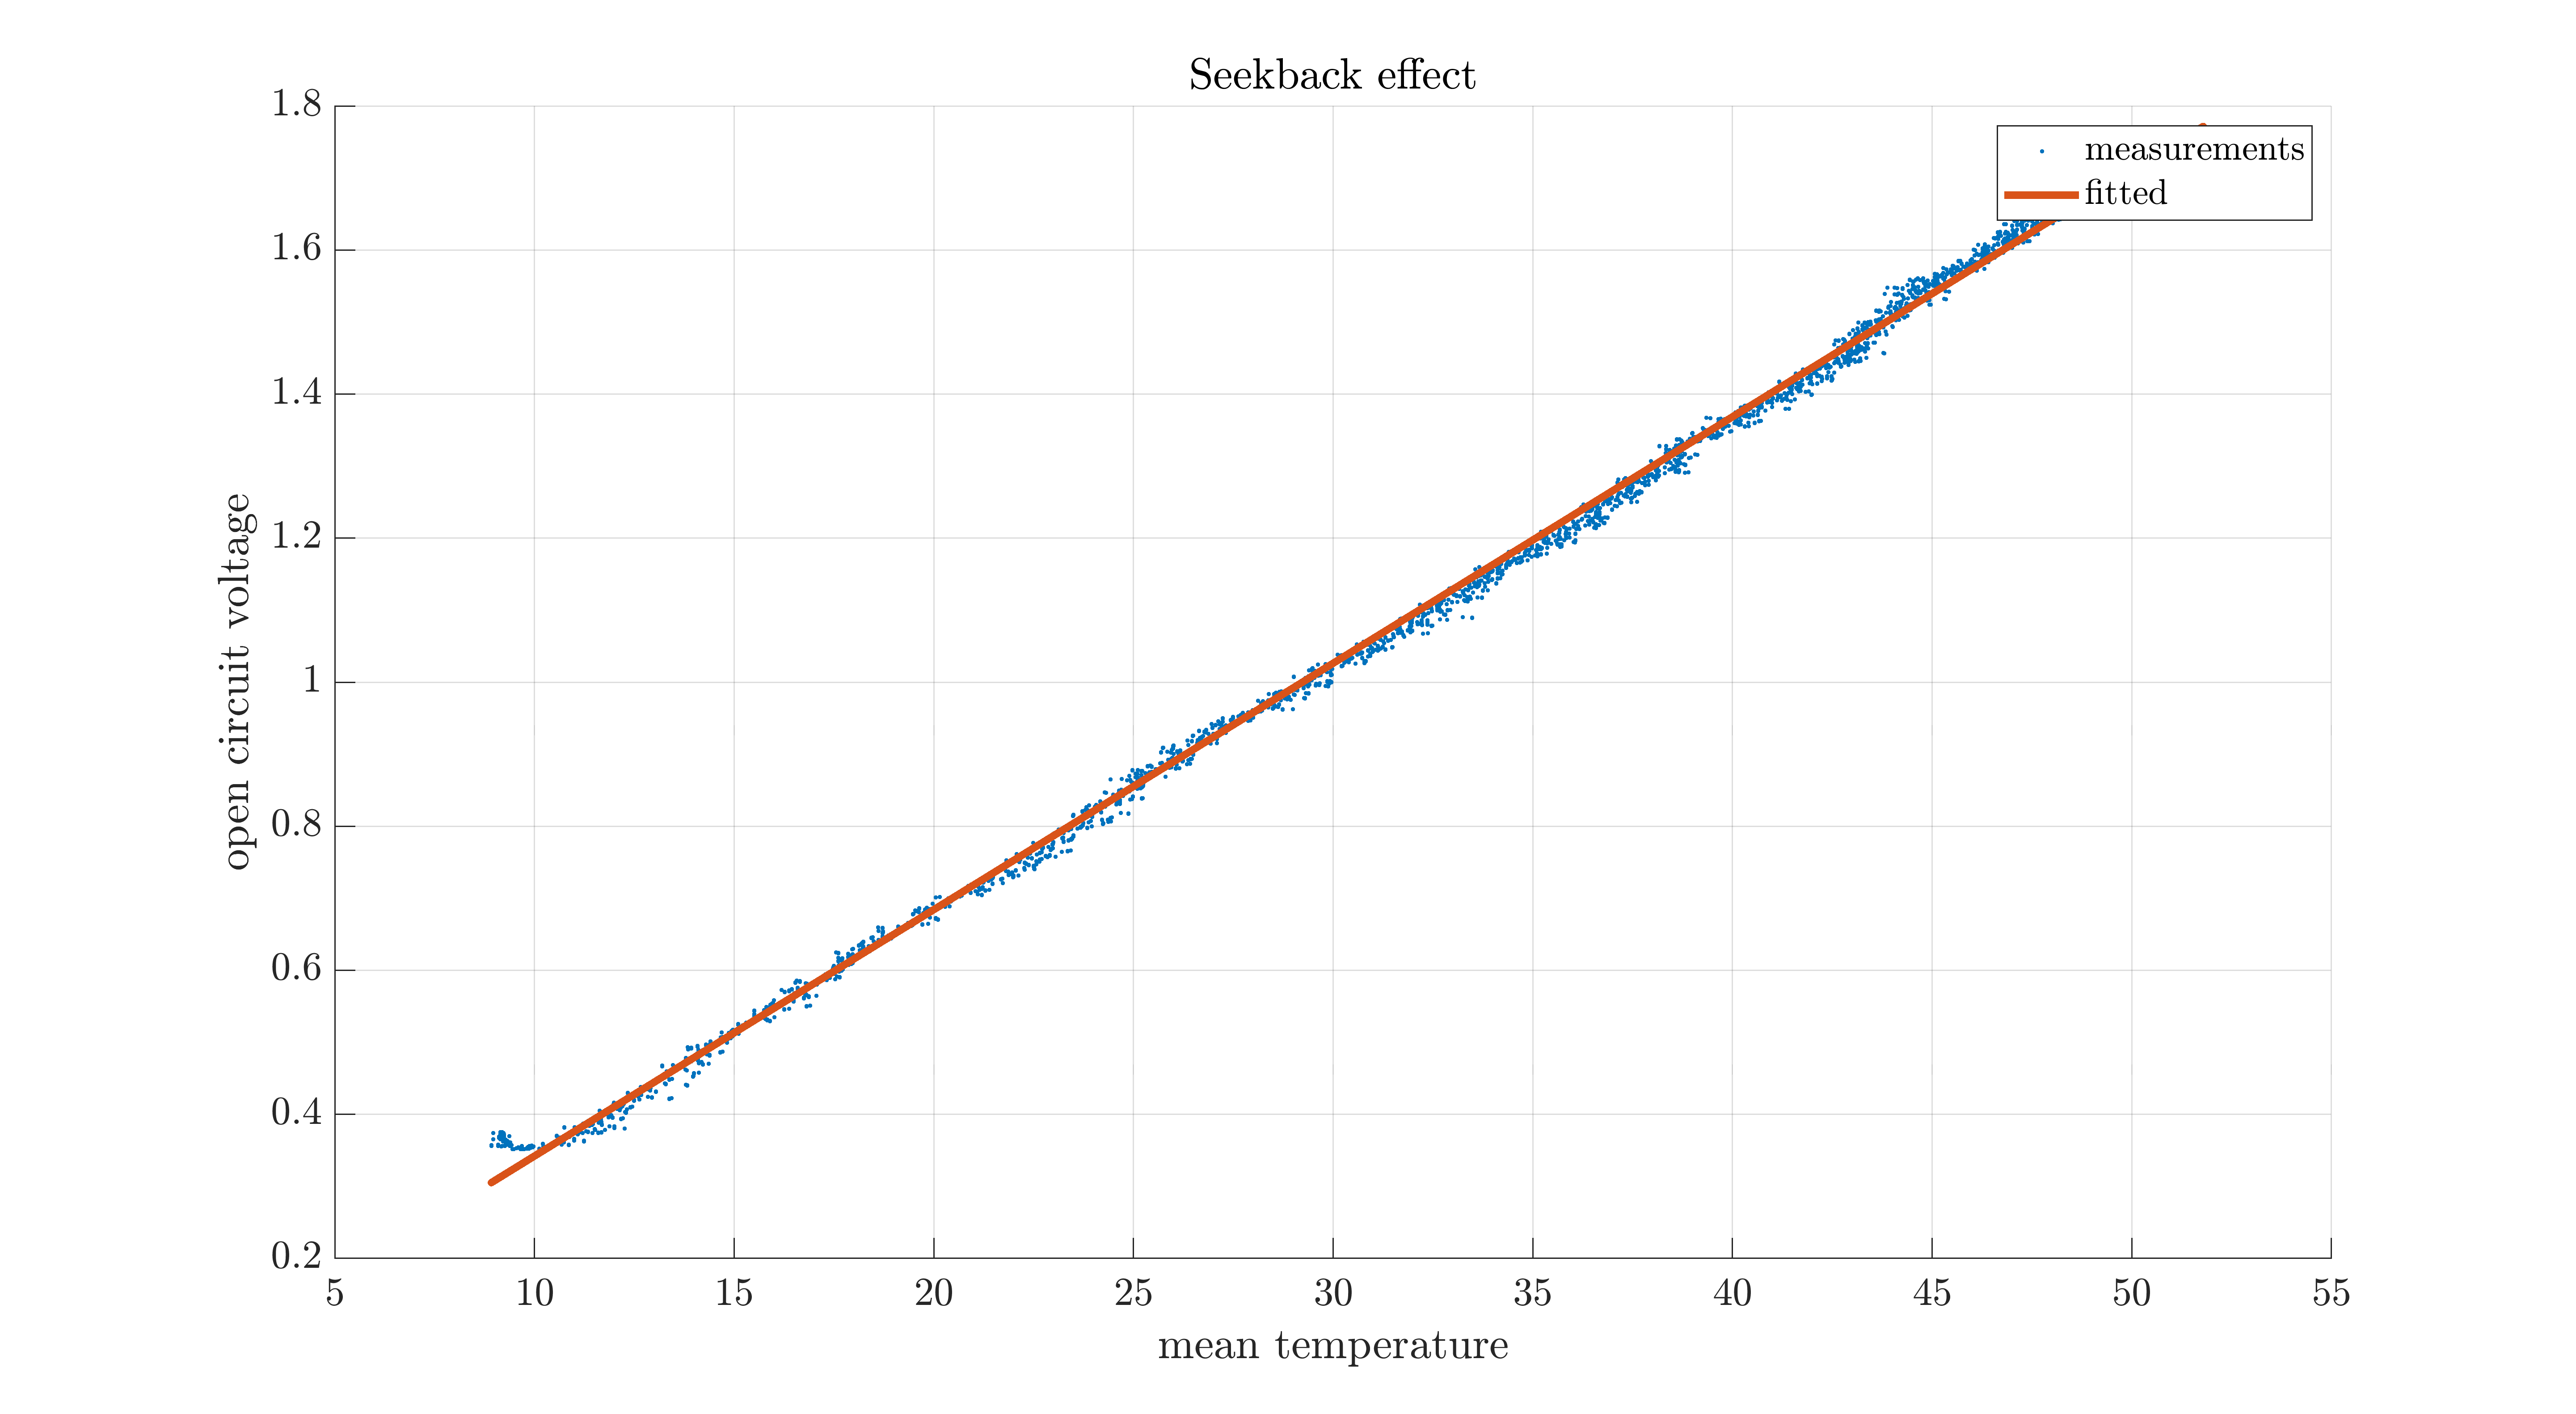
\includegraphics[width=0.45\textwidth]{assets/Seekback effect.png}
    \caption{Open circuit voltage mean temperature dependence}
    \label{fig:voc_dep_t}
\end{figure}
\begin{figure}[h]
    \centering
    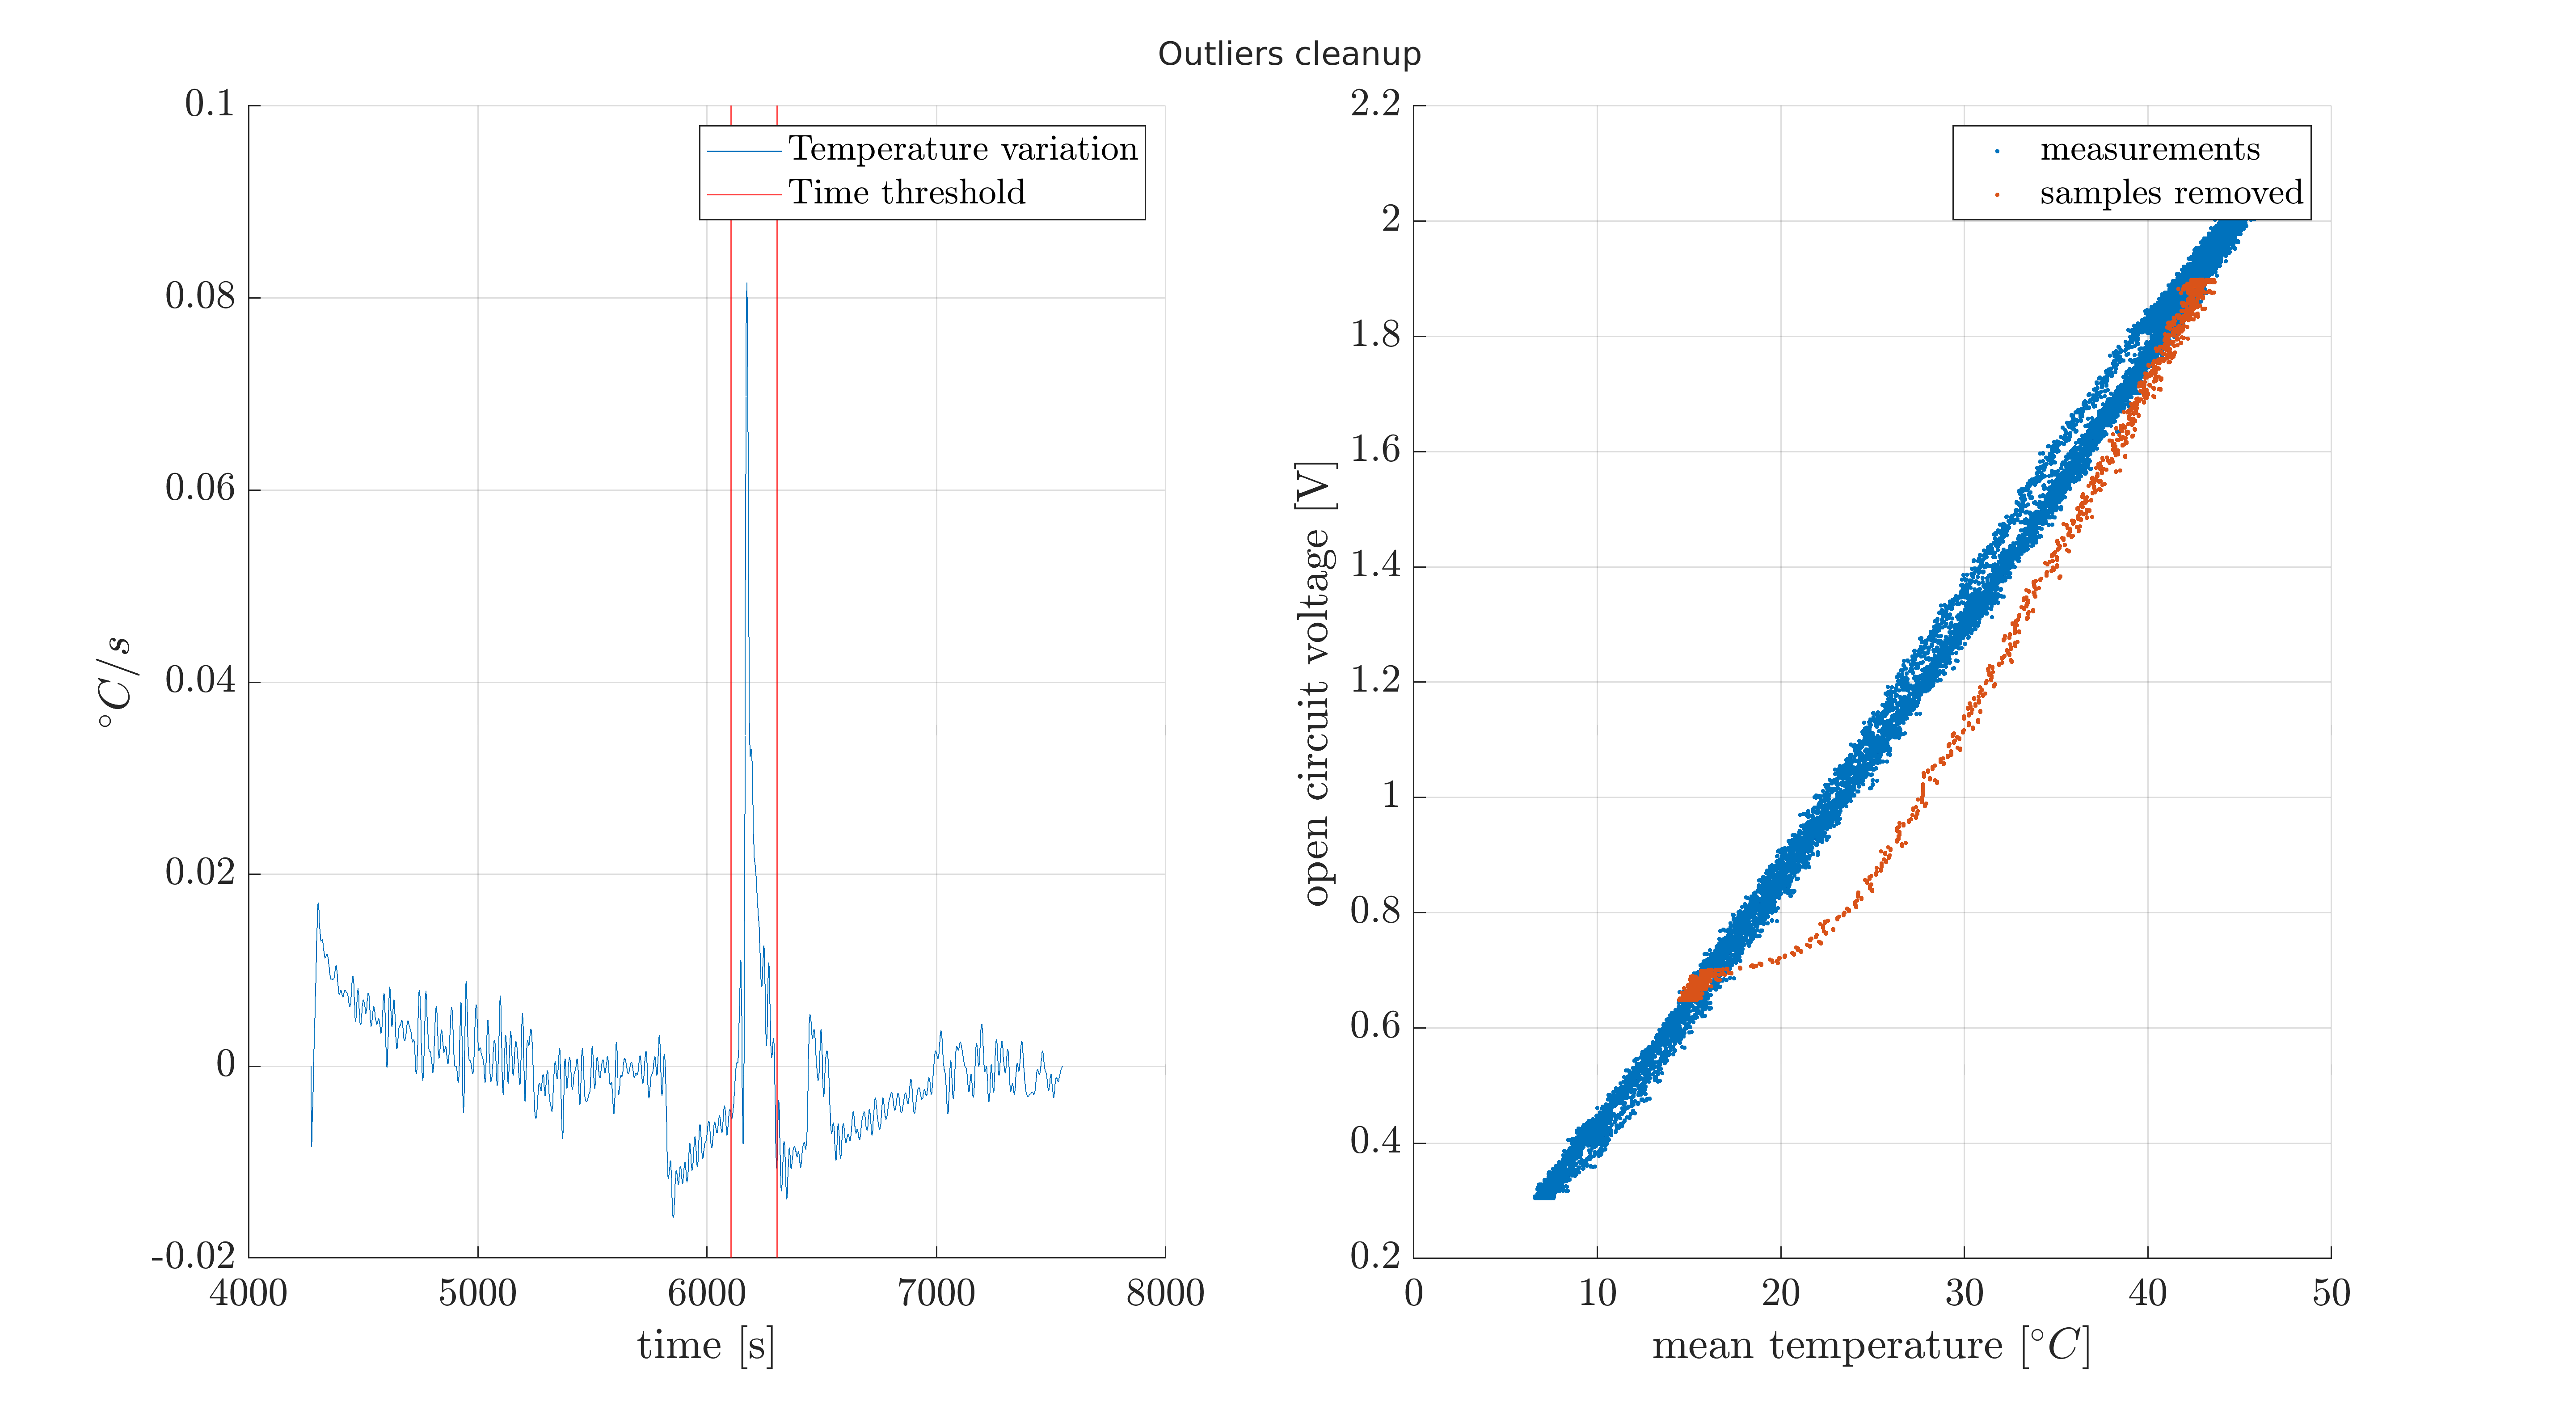
\includegraphics[width=0.45\textwidth]{assets/Outliers cleanup.png}
    \caption{Cleanup of outliers from an experiment contaimnation.}
    \label{fig:voc_cleanup}
\end{figure}

% Come raffigurato in figura\ref{fig:voc_dep_t}, dal momento che i dati non sono sovrapposti a una linea, sembrerebbe che il coefficiente di Seebeck non sia dipendente solamente dalla differenza di temperatura, ma anche dalla temperatura media. Questo tuttavia non è vero, perché il coefficiente di Seeback è di per sè una costante del materiale e dalla forma. Per questo motivo, abbiamo analizzato i dati focalizzandoci sulla variazione della temperatura media nel tempo, quindi filtrata e derivata rispetto al tempo. Il risultato mostra un picco nella variazione di temperatura, causato da qualche evento esterno che ha contaminato le letture. Abbiamo quindi tolto gli outliers e rifatto il fitting, con i risultati mostrati in figura \ref{fig:voc_cleanup}

An anomaly in the data stands out. As depicted in figure\ref{fig:voc_dep_t}, since the data are not superimposed on a line, it would appear that the Seebeck coefficient is not only dependent on the temperature difference, but also on the mean temperature. However, this is not true, because the Seeback coefficient is itself a constant of the material and from the shape. For this reason, we analyzed the data by focusing on the change in mean temperature over time, then filtered and derived with respect to time. The result shows a spike in the temperature variation, caused by some external event that contaminated the readings. We then removed the outliers and ran again the fitting, with the results shown in Figure \ref{fig:voc_cleanup}.


% Sappiamo che la scelta scientificamente più corretta sarebbe stato ripetere l'esperimento, ma raccogliere dati del tutto precisi è molto complicato, ci siamo accorti di questo problema solo in fase di analisi e togliendo lo spike di errore sono dati comunque validi.

% The Seeback coefficient is in itself a polynomial which is dependent on the mean temperature, this contribution was added after noticing that in a plot with measured voltage dependent on delta temperature, the data was not lying on a line, but seemed to have a dependency on mean temperature. Since Seeback coeeficient is a material and shape constant, it should be not dependent on mean temperature. To addess this problem we analyzed the single event that could have caused the wrong readings. In particular we focused on the variation of mean temperature in time, so we filtered the readings and differentiated it with respect to time, the result shows a spike in the temperature variation. This behaviour was caused by some external event that contaminated the readings. We then removed the outliers and the fit was done again, the result is shown in figure \ref{fig:voc_cleanup}.

\subsection{Fitting internal resistance}
We modeled the internal resistance as a constant plus a linear term dependent on the mean temperature. 
The equations used to fit the model are:
\begin{align}
    \begin{split}
    R_{int} &= R_{int_0} + R_{int_1} \cdot \overline{T} \\
    V_{OC} &= S \cdot \Delta T \\
    I &= \frac{V_{OC}}{R_{int} + R_{load}}
    \end{split}
\end{align}
The internal resistance was fitted with the following MATLAB code:

\begin{lstlisting}[
    frame=single,
    numbers=none,
    style=Matlab-editor,
    basicstyle=\tiny,
]
% Model of internal resistance
internal_resistance_mdl = @(internal_resistance_coeffs, mT_dT)(internal_resistance_coeffs(1) + internal_resistance_coeffs(2) * mT_dT(:,1));
% Model of current given a load resistance value
current_mdl = @(internal_resistance_coeffs, mT_dT_Voc)(mT_dT_Voc(:,3) ./ (load_value + internal_resistance_mdl(internal_resistance_coeffs, [mT_dT_Voc(:,1), mT_dT_Voc(:,2)])));

% Define residuals function (RMSE)
residuals = @(coeffs)(residuals_function(I, current_mdl(coeffs, [mT, dT, Voc])));

% Minimize residuals with contraints
default_options = optimoptions('fmincon');
fitted_internal_resistance_coeffs = fmincon(residuals, [0.5, 0],[],[],[],[], [0, 0], [5, inf], [], default_options);
\end{lstlisting}

\begin{figure}[h]
    \centering
    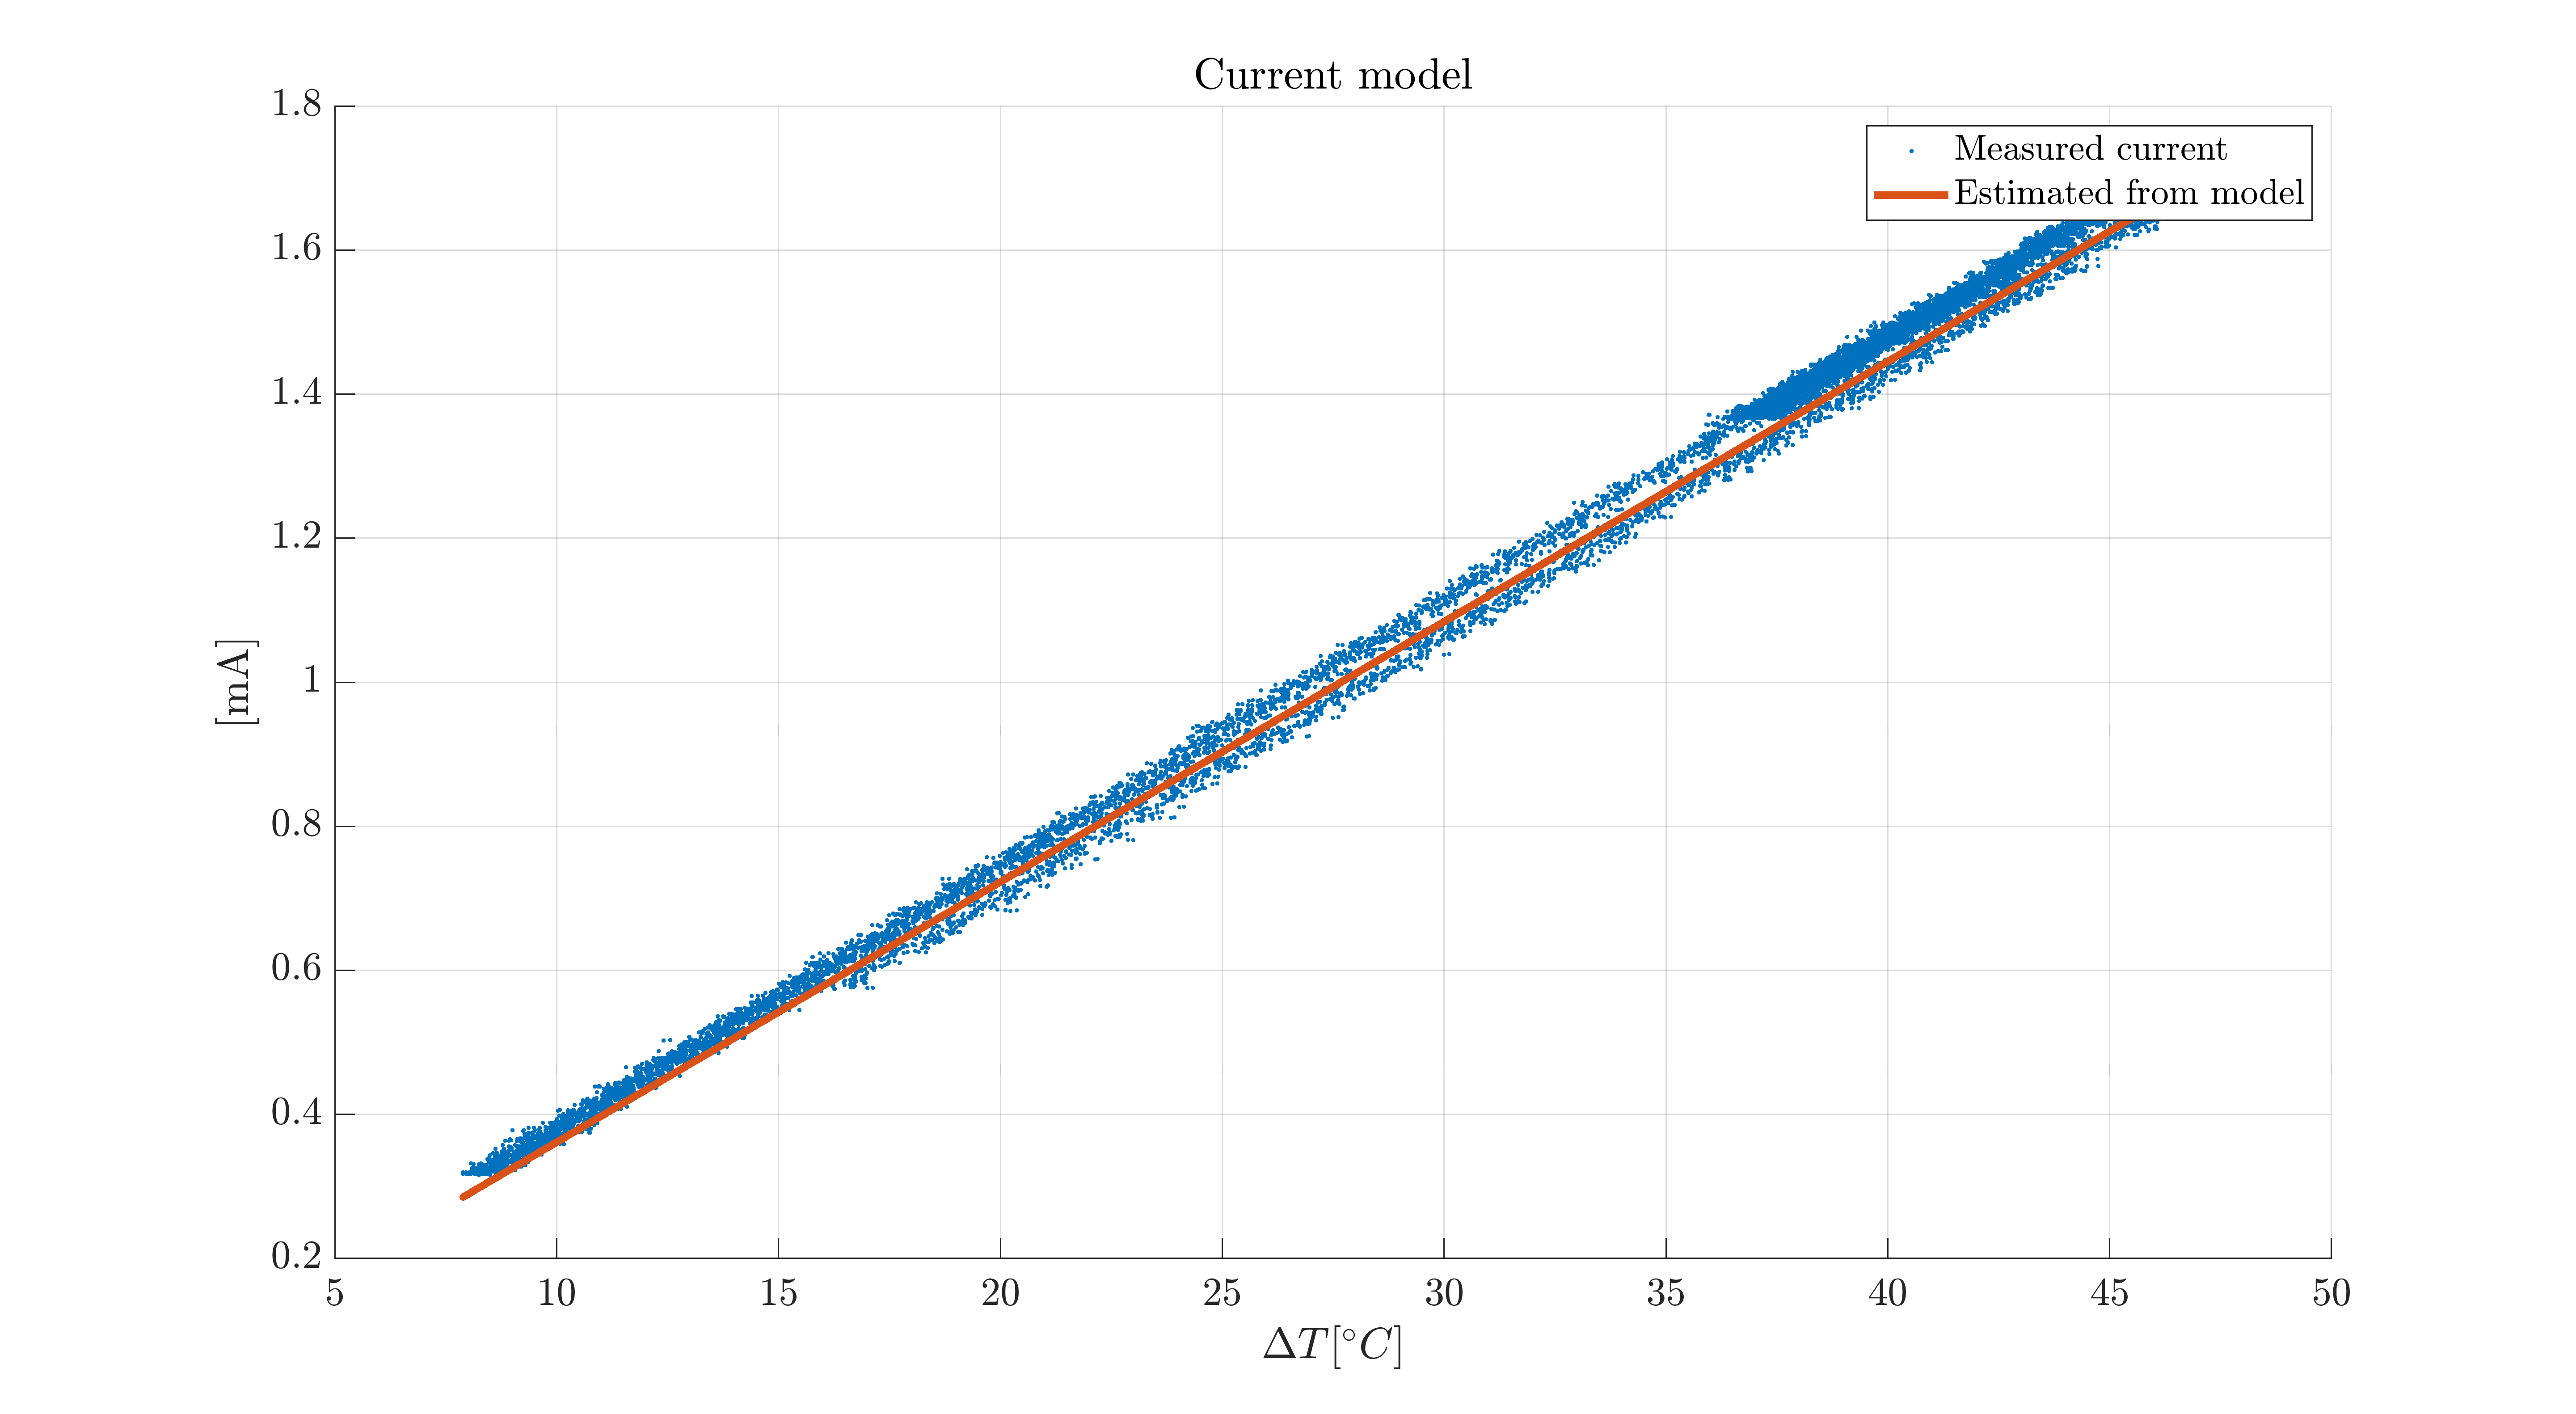
\includegraphics[width=0.45\textwidth]{assets/Current model.png}
    \caption{Measured current vs model estimate.}
    \label{fig:voc_current_model}
\end{figure}


\section{Conclusion}
% The conclusion goes here.
% Usually, the conclusion takes 15-20 lines (less than half a column) and should resume your told story.
% \\
% \\
% Context/Scenario  $\Rightarrow$  Challenges  $\Rightarrow$\\
%  $\Rightarrow$ What you have done $\Rightarrow$ \\
%  $\Rightarrow$ most important achievements, with key numbers. 
% \\
% Moreover, you could add short anticipation of advisable future works and directions to improve or to extend the project (beyond your task).  
% \\
% \\
% For more information, please refer to~\cite{IEEEexample:IEEEwebsite}. For \LaTeX~   information, you can have a look to~\cite{IEEEhowto:IEEEtranpage}  (Anyway \LaTeX~   is not mandatory).
% \\
% I wish you the best of success.

% In our project, we were able to find the internal resistance and Seebeck coefficient of the flexible fibre-based TEG. Due to a lack of the needed instrumentation, we were unable to collect the necessary data to determine the thermal conductivity. However, it can be obtained by measuring the efficiency. We know that the maximum efficiency of the TEG is achieved by matching impedance and internal resistance. Knowing the internal resistance, we can then find the maximum efficiency, from which we derive the figure of merit and the thermal conductivity.

We made measurements on three different types of TEG. The first two are classical TEG modules, and fitted results are in line with the online datasheets. The last one is a fibre-based TEG.\\

\vspace{5mm}

\begin{tabular}{ |p{2cm}|p{2.2cm}|p{2.2cm}|  }
    \hline
    TEG model & Seebeck & Internal resistance\\
    \hline
    TEG MAT & 0.034209 & 0.145028, 0.001342\\
    \hline
    TEG 12706 & 0.044441 & 2.299155, 0.083479\\
    \hline
    TEG VL25  & 0.007100 & 0.511499, 0.004171\\
    \hline
\end{tabular}

\vspace{5mm}

From the results obtained, the best TEG is the TEG MAT, having the highest Seeback coefficient and lowest internal resistance. Here is the link to the \href{https://github.com/gmazzucchi/tegc}{project repository}. In our project, we determined the internal resistance and Seebeck coefficient of the flexible fiber-based TEG. However, due to the unavailability of the requisite instrumentation, we were unable to collect the necessary data for determining the thermal conductivity. Nonetheless, this can be achieved by measuring the efficiency, as it is known that the maximum efficiency of the TEG is achieved by matching impedance and internal resistance. By determining the internal resistance, we can subsequently obtain the maximum efficiency, and thereby derive the figure of merit and the thermal conductivity.\\
In the future, it would be preferable to avoid setting temperatures manually. Instead, a cycle of temperatures should be set automatically by the microcontroller. This will allow for greater homogeneity in the dataset.




% if have a single appendix:
%\appendix[Proof of the Zonklar Equations]
% or
%\appendix  % for no appendix heading
% do not use \section anymore after \appendix, only \section*
% is possibly needed

% use appendices with more than one appendix
% then use \section to start each appendix
% you must declare a \section before using any
% \subsection or using \label (\appendices by itself
% starts a section numbered zero.)
%


% \appendices
% \section{Proof of the First Zonklar Equation}
% Appendix one text goes here.

% % you can choose not to have a title for an appendix
% % if you want by leaving the argument blank
% \section{}
% Appendix two text goes here.


% % use section* for acknowledgment
% \section*{Acknowledgment}


% The authors would like to thank...


% Can use something like this to put references on a page
% by themselves when using endfloat and the captionsoff option.
\ifCLASSOPTIONcaptionsoff
  \newpage
\fi



% trigger a \newpage just before the given reference
% number - used to balance the columns on the last page
% adjust value as needed - may need to be readjusted if
% the document is modified later
%\IEEEtriggeratref{8}
% The "triggered" command can be changed if desired:
%\IEEEtriggercmd{\enlargethispage{-5in}}

% references section

% can use a bibliography generated by BibTeX as a .bbl file
% BibTeX documentation can be easily obtained at:
% http://mirror.ctan.org/biblio/bibtex/contrib/doc/
% The IEEEtran BibTeX style support page is at:
% http://www.michaelshell.org/tex/ieeetran/bibtex/
%\bibliographystyle{IEEEtran}
% argument is your BibTeX string definitions and bibliography database(s)
%\bibliography{IEEEabrv,../bib/paper}
%
% <OR> manually copy in the resultant .bbl file
% set second argument of \begin to the number of references
% % (used to reserve space for the reference number labels box)
% \begin{thebibliography}{1}

% \bibitem{IEEEhowto:kopka}
% H.~Kopka and P.~W. Daly, \emph{A Guide to \LaTeX}, 3rd~ed.\hskip 1em plus
%   0.5em minus 0.4em\relax Harlow, England: Addison-Wesley, 1999.

% \end{thebibliography}

\bibliographystyle{./IEEEtran}
\bibliography{./IEEEabrv,./IEEEexample,./references/experimental_characterization,./references/flexible_tegc,./references/tegc_load_dependence,./references/tegc_waste_heat_recovery,./references/thermoelectricgenerator,./references/modeling-of-a-thermoelectric-generator-device.bib}





% biography section
% 
% If you have an EPS/PDF photo (graphicx package needed) extra braces are
% needed around the contents of the optional argument to biography to prevent
% the LaTeX parser from getting confused when it sees the complicated
% \includegraphics command within an optional argument. (You could create
% your own custom macro containing the \includegraphics command to make things
% simpler here.)
%\begin{IEEEbiography}[{\includegraphics[width=1in,height=1.25in,clip,keepaspectratio]{mshell}}]{Michael Shell}
% or if you just want to reserve a space for a photo:

% \begin{IEEEbiography}{Michael Shell}
% Biography text here.
% \end{IEEEbiography}

% % if you will not have a photo at all:
% \begin{IEEEbiographynophoto}{John Doe}
% Biography text here.
% \end{IEEEbiographynophoto}

% % insert where needed to balance the two columns on the last page with
% % biographies
% %\newpage

% \begin{IEEEbiographynophoto}{Jane Doe}
% Biography text here.
% \end{IEEEbiographynophoto}

% % You can push biographies down or up by placing
% % a \vfill before or after them. The appropriate
% % use of \vfill depends on what kind of text is
% on the last page and whether or not the columns
% are being equalized.

%\vfill

% Can be used to pull up biographies so that the bottom of the last one
% is flush with the other column.
%\enlargethispage{-5in}



% that's all folks
\end{document}


